\section{Evaluation}
\label{sec:evaluation}

\subsection{Setup}

\subsubsection{Metrics}
In our evaluation we are investigating several metrics:

\begin{enumerate}
\setlength{\itemsep}{-3pt}  

\item the power consumption of the system

\item the recall of the event of interest

\item the precision of event of interest detection

\item the time delay incurred before the application becomes aware that an event of interest has occurred

\item the precision of device wake-ups

\end{enumerate}

Recall is the fraction of events of interest that have been successfully detected. We calculate event of interest recall by dividing the number of true positives by the total number of events of interest in the baseline (usually groud truth). Precision is the fraction of the detected events of interest that are present in the baseline. For a particular event of interest we calculate precision by dividing the number of true positives by the number of detected events of interest of that type. Device wake-up precision is a measure of how often the device unnecessarily wakes up (i.e. wakes up and does not detect an event of interest).

\subsubsection{Simulator}

To ensure repeatability across different experimental runs we use accelerometer traces 
captured ahead of time as the input data. Each trace is an ordered set of accelerometer 
readings. Each reading contains the x-, y- and z-components of the acceleration vector and 
a timestamp indicating the time when the reading was produced.

In our benchmarks we are looking to obtain results for a multitude of wake-up approaches, each with up to four independent parameters. In order to reduce the impact of outliers on our results we wanted to run each benchmark on a multitude of similarly-generated accelerator traces. The combination of all traces and parameterized wake-up approaches resulted in over 200,000 runs. With each trace being at least half an hour long, it would have been infeasible to perform all the runs online. The alternative was to create a simulator that processes the collected acceletometer traces offline. 

For each run, the simluator takes the following inputs:

\begin{enumerate}
\setlength{\itemsep}{-3pt}  

\item a parametarized wake-up approach

\item a file containing the accelerometer readings, sorted by timestamp

\item a file containing information about ground truth

\end{enumerate}

The simulator processes the readings one at a time, similarly to how a mobile device would receive accelerometer readings in real-time, as they are produced by the sensor. Based on the wake-up approach, the simulator determines which of the readings would cause the device to wake-up. Also, the simulator determines what reading need to be sent to the running application(s). At the end of the run, the simulator output relevant metrics such as:

\begin{enumerate}
\setlength{\itemsep}{-3pt}  

\item amount of time the device would have been awake

\item total number of device wake-up

\item number of wake-ups that did not result in an event of interest being detected

\item true positives, false positives and false negatives

\item event of interest recall and precision

\end{enumerate}

\subsubsection{Power Consumption Model}

To complement our simulator, we created a model to estimate the power consumption for each of our simulator runs. The model is based on real power measurements presented in 
subsection \ref{subsec:power_consumption_values}. The inputs of the model are the amount 
of time the device is awake, the amount of time it is asleep and the number of transitions 
between the two states. Based on these values, the energy model outputs the
average power consumption over the duration of the trace.

\subsection{Power Consumption Values} \label{subsec:power_consumption_values}

We performed power measurements on a Google Nexus 4 running Android 4.2.2. The
results are summarized in Table \ref{table:powerMeasurements}. 

We evaluated two options as our low-powered sensor platform. Our first option is a Texas Instruments
MSP430 microcontroller. It has the advantage of being very low-power, but it has limited memory and
cannot perform complex analysis of sensor data in real-time. Our second option is a Texas Instruments
Stellaris LM4F120H5QR microcontroller powered by a Cortex-M4 CPU. It can batch a higher number of
readings and perform more complex data analysis, but it has a bigger energy footprint. The power
measurements for both microcontrollers are also presented in Table \ref{table:powerMeasurements} on page \pageref{table:powerMeasurements} .

TODO: mention that power measurements were taken with sceen off, GSM off, WiFi off, GPS off (and explain why) 
\begin{table*}[t]
\begin{tabular}{| l | p{7cm} | l | l |}
    \hline
    Device & State & Average Power Consumption (mW) & Average Duration \\ \hline
    TI MSP430 & Awake & 3.6 & N/A \\ \hline
    TI Stellaris & Awake & 49.4 & N/A \\ \hline
    Nexus 4 & Awake, running an application with data from the internal accelerometer & 323 & N/A \\ \hline
    Nexus 4 & Asleep & 9.7 & N/A \\ \hline
    Nexus 4 & Asleep-to-Awake Transition & 384 & 1 second \\ \hline
    Nexus 4 & Awake-to-Asleep Transition & 341 & 1 second \\ \hline
\end{tabular}
\caption{Power Measurements}
\label{table:powerMeasurements}
\end{table*}
    

\subsection{Microbenchmarks}

\subsubsection{Setup}
To collect the accelerometer traces for our microbenchmarks we used an AIBO TODO:model robot. The robot would perform a sequence of actions (a circuit) and record timestamps for the beginning and end of each action. The set of performed actions and timestamps were outputed to a log file that can be used by the simulator as ground truth. To record the accelerometer trace, we attached a Google Nexus 4 to the back of the dog and ran an application that collected all the accelerometer reading for the duration of the circuit.

For these microbenchmarks, we implemented 3 applications that attempt to detect 4 different actions from the acceleromter readings in each trace. A first application looks for local maxima within a certain range in the x-axis acceleration to detect step taken by the robot. Similarly, the second application looks for local minima within a range in the y-axis acceleration to detect headbutt motions. The third application monitors changes in the acceleration due to gravity on the y and z axes in order to detect stance transitions between a normal posture and sitting. All 3 applications pass the data they are interested in through low-pass filters based on Fast-Fourier Transformations.

The level of activity can vary significantly between mobile device users. For example, the mobile device of an individual working in an office environment may experience low levels of motion (e.g. sitting on a desk for extended periods of time), while the mobile device of someone constantly in motion (e.g. bike courier) may only experience short period at rest. In our microbenchmarks we wanted to cover a wide range of activity level. We divided our traces into 3 groups based on activity level. Groups 1, 2 and 3 contain traces in which the robot performs actions approximately 10\%, 50\% and 90\% of the time, respectively. Within each trace, we also wanted the amount of time each action type is being performed to vary considerably. Figure \ref{fig:actionTimes} shows the average amount of time each action is being perform for the traces in each group, as a percentage of the average trace length. 

\subsubsection{Always Awake}

In the Always Awake approach, the device is presumed to be awake for the entire duration of the trace and all of the collected accelerometer readings are passed to the applications. We are using the Always Awake approach as a baseline to compare all the following wake-up approaches. Additionally, the Always Awake simulations show the accuracy of the implemented applications in terms of event of interest detection precision and recall. Figure \ref{fig:aaRecallByGroup} shows the recall of each of the events of interest averaged over the traces in each group. We note that with the exception of the headbutt action in Group 1, the event of interest recall is above 95\% for all actions and groups. The headbutt action in group 1 appears to be an outlier because Group 1 contains traces with the least amount of actions and headbutts are the scarcest actions, occurring only about once per trace. Figure \ref{fig:aaPrecisionByGroup2} shows the detection precision of each of the events of interest averaged over the traces in each group. For all cases, the applications achieved a detection precision above 82\%.

The power consumption using this approach is equivalent to the power consumed by the device in the awake state. In the case of the Nexus 4 used in our experiments, the power consumption is 323 mW, as shown in Table \ref{table:powerMeasurements}.

\subsubsection{Duty Cycling}

In the Duty Cycling wake-up approach, the device is set to wake-up at regular time intervals and caputure several seconds of accelerometer readings. If an event of interest is detected based on those readings, the device will continue capturing sensor data until events of interest are not being detected anymore. 

This approach comes with several drawbacks. As shown in Figure \ref{fig:dcRecallByInterval}, recall drops dramatically as the wake-up interval is increased because more events of interest are being missed while the device is sleeping. Figure \ref{fig:dcRecallVsPower} shows the relationship between power consumption and recall. While duty cycling can achieve significant power savings, it does so at the expense of recall. Additionally, if the event of interest happens rarely, as it is the case of group 1, duty cycling becomes inefficient bacause it causes many unnecessary wake-ups. Figure \ref{fig:dcWakeUpPrecisionByInterval} shows that for Group 1, only about 1 in 9 wake-ups result in an event of interest being detected, regradless of the wake-up interval.

A duty cycling wake-up approach is not appropriate for applications that require a high event of interest recall, such as a fall detector or a gesture recognizer.

\subsubsection{Batching and Duty Cycling}

In the Batching and Duty Cycling approach, the device uses a peripheral processor to collect all the available sensor data while the main processor is asleep. As in the duty cycling approach, the main processor is set to wake up at regular intervals. After each wake-up, the main processor fetches the entire batch of sensor readings from the peripheral processor and passes it to each of the applications. The net result is no loss in recall compared to the Always Awake case because the applications receive all the sensor readings. 

Our simulations, sumarized in Figure \ref{fig:batchingPowerByInterval} indicates that power savings can be achieved for wake-up intervals greater than 5 seconds. Shorter wake-up intervals can potentially cause more energy consumption than the Always Awake case because of the additional energy cost of transitioning between the sleep and awake states. Note that increasing the wake-up interval has diminishing power saving returns. A lower bound to the power consumption of the entire system is the sum of the power consumed by the main device while sleeping and the peripheral processor while being awake.

Similarly to the duty cycling approach, this approach can be inefficient if the event of interest occurs infrequently because of a high number of unnecessary wake ups. Figure \ref{fig:batchingWakeUpPrevisionByInterval} shows that, for group 1, even for a wake-up interval as high as 30 seconds, this approach does not achieve a wake-up precision over 40\%. That is, less than 2 out 5 wake-ups result in an event of interest being detected.

In this approach, events of interest are only detected after the main processor wakes up. As a result, the delay between the time when the event is occuring and the time when it is detected can be as long as the batching interval. Therefore, this approach may not be appropriate for applications that are expected to react immediately after an event of interest occurs. For example, the user of a gesture recognition application would not be satisfied if the application detects the performed gesture after a delay of more than a couple of seconds.


\subsubsection{Wake-up Conditions}

In the wake-up conditions approach, the peripheral processor anylises the sensor data in order to determine if it satisfies a specific wake-up condition. If the condition is specified the main processor is woken up and passed all the sensor data until the condition stops being satisfied. Our goal for the wake-up conditions approach was to attempt to achieve power savings with little or no impact on recall and detection timeliness. 

The first question we tried to answer was whether or not a static wake-up condition would be good enough to achieve our goal. It quickly became apparent that this was not the case. We can achieve very high recall if we use a leniant wake-up condition such as one that is satisfied whenever any motion is detected. Unsurprisingly, this is inefficient if we are only interested in a small portion of the occuring events. For example, if we were only interested in detecting headbutts, we don't want the main processor to wake-up every time the robot was walking or transitioning between stances. More often than not, the wake-up condition cannot be static. Each application should be able to specify its own wake-up condition. Otherwise, the system might not achieve high enough recall or any significant power savings.



\subsection{Macrobenchmarks}

\subsubsection{Setup}
For the macrobenchmarks, we implemented a pedometer application that attemps to detect steps, as described in TODO:cite pedometer paper. This application differs slightly from the step detector implemented for our microbenchmarks. Firstly, this application looks at the entire acceleration magnitide, rather than just the acceleration on the x-axis. This change was necessary because the user may orient the device in any position, rather than having a fixed orientation as was the case with the device attached to the robot. Secondly, some sensitivity parameters had to be adjusted because human walking generates significantly more acceleration that the robot. 

The traces were captured by three different people performing routine daily activities. The first trace is 2 hours and 10 minutes long captured during a person's morning commute. The trace is approximately a 30-70 split between walking and riding a train, respectively. The second trace is 1 hour and 2 minutes long and captured by a person working in a retail store. Most of the trace is spent interacting with customers. The third trace is 3 hours and 17 minutes long, captured by a person working in an office environment. Approximately 10\% of traces 2 and 3 are spent walking.

TODO:Describe how recall and precision are calculated (i.e. compared to always awake baseline)

\subsubsection{Always Awake}

\subsubsection{Duty Cycling}

\subsubsection{Batching and Duty Cycling}

\subsubsection{Wake-up Conditions}

\begin{figure}[p]
	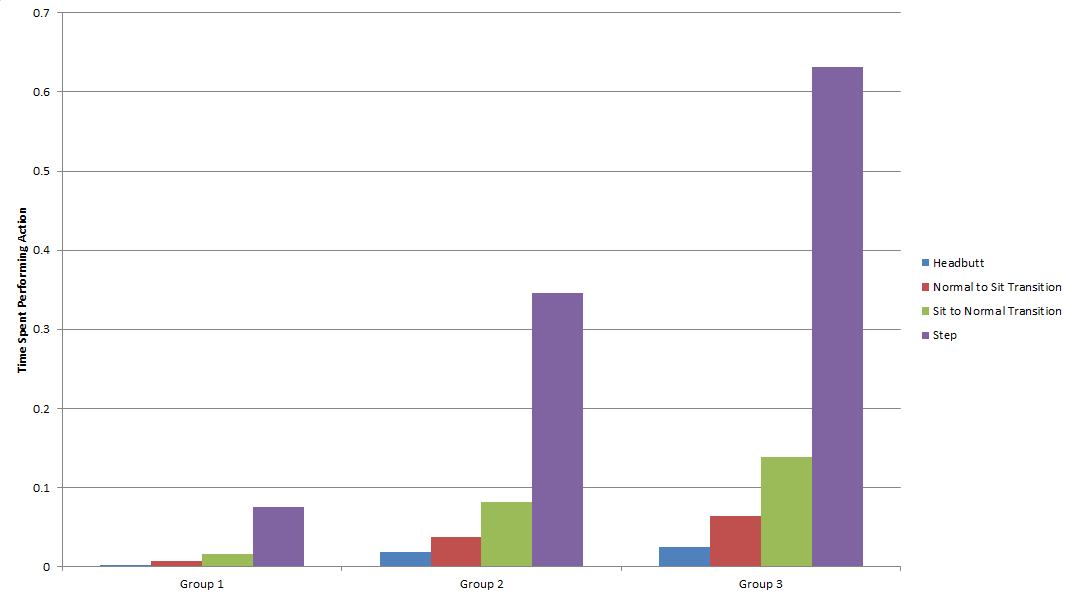
\includegraphics[width=9cm]{action_times.png}
	\caption{Time spent performing actions of specific types as a percentage or trace length}
    	\label{fig:actionTimes}
\end{figure}

\begin{figure}[p]
	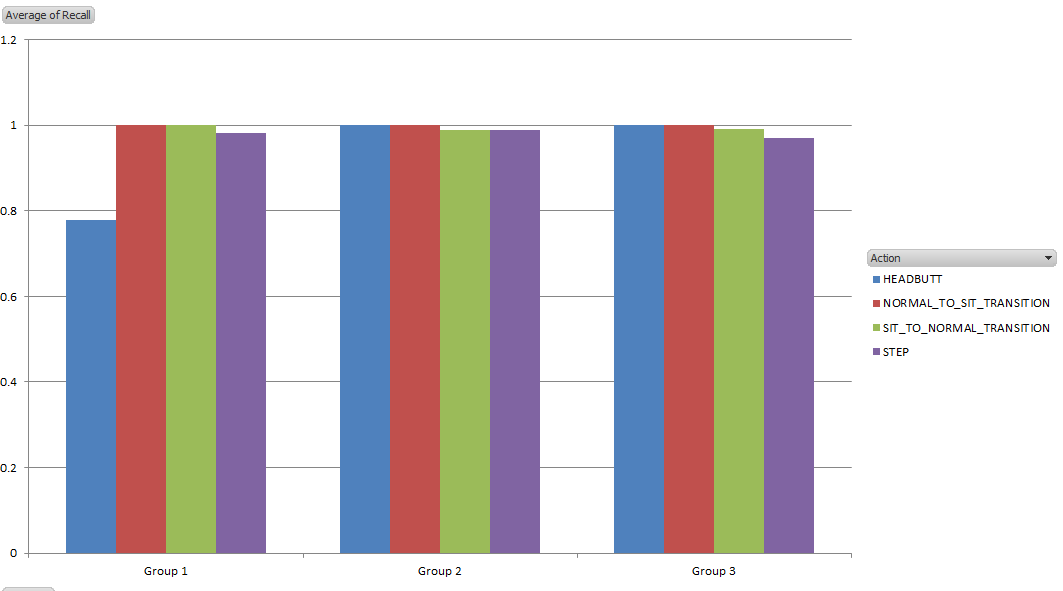
\includegraphics[width=9cm]{aa_recall_by_group.png}
	\caption{Always Awake: Recall by Group}
    	\label{fig:aaRecallByGroup}
\end{figure}


\begin{figure}[p]
	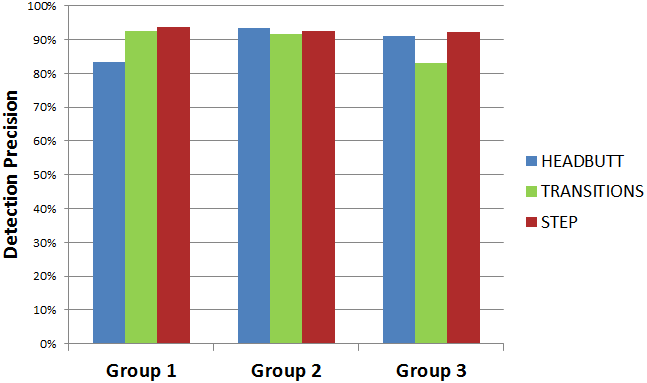
\includegraphics[width=9cm]{aa_precision_by_group.png}
	\caption{Always Awake: Detection Precision by Group}
    	\label{fig:aaPrecisionByGroup}
\end{figure}


\begin{figure}[p]
	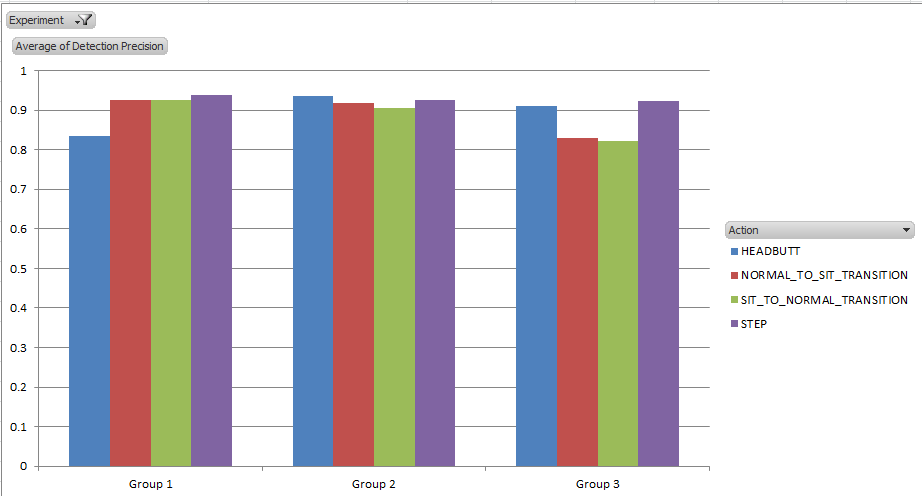
\includegraphics[width=9cm]{aa_precision_by_group2.png}
	\caption{Always Awake: Detection Precision by Group}
    	\label{fig:aaPrecisionByGroup2}
\end{figure}


\begin{figure}[p]
	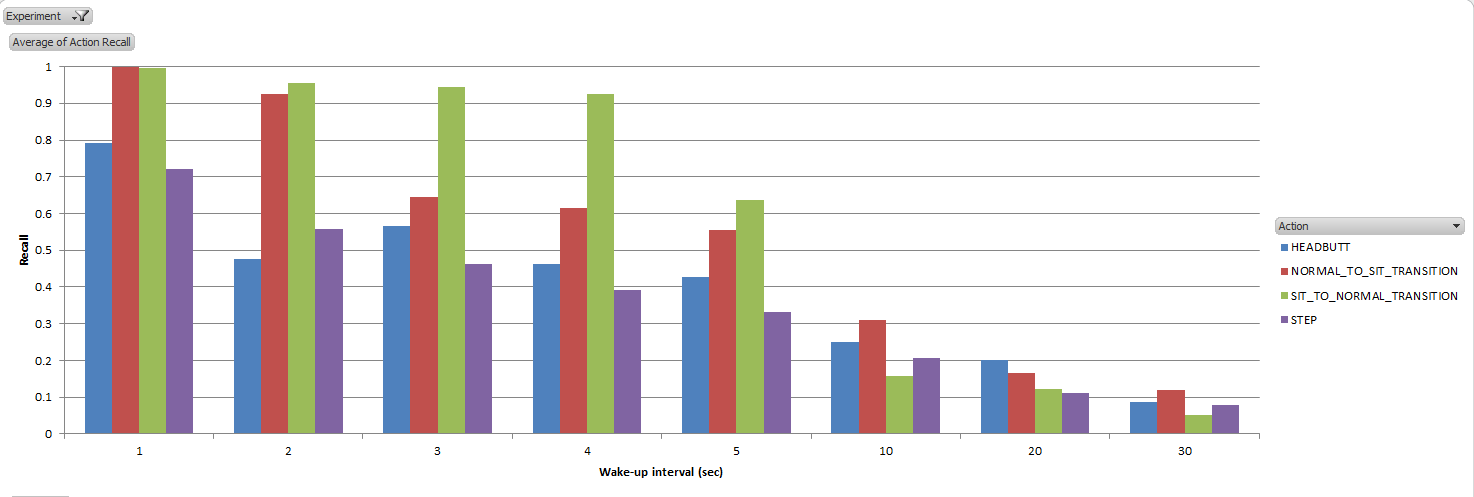
\includegraphics[width=9cm]{dc_recall_by_interval.png}
	\caption{Duty Cycling: Recall by Wake-up Interval}
    	\label{fig:dcRecallByInterval}
\end{figure}


\begin{figure}[p]
	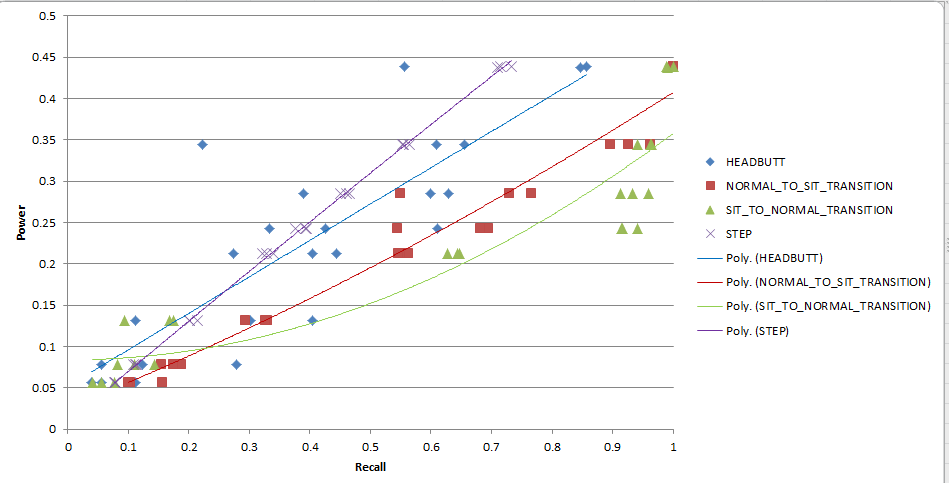
\includegraphics[width=9cm]{dc_recall_vs_power.png}
	\caption{Duty Cycling: Recall vs Power}
    	\label{fig:dcRecallVsPower}
\end{figure}


\begin{figure}[p]
	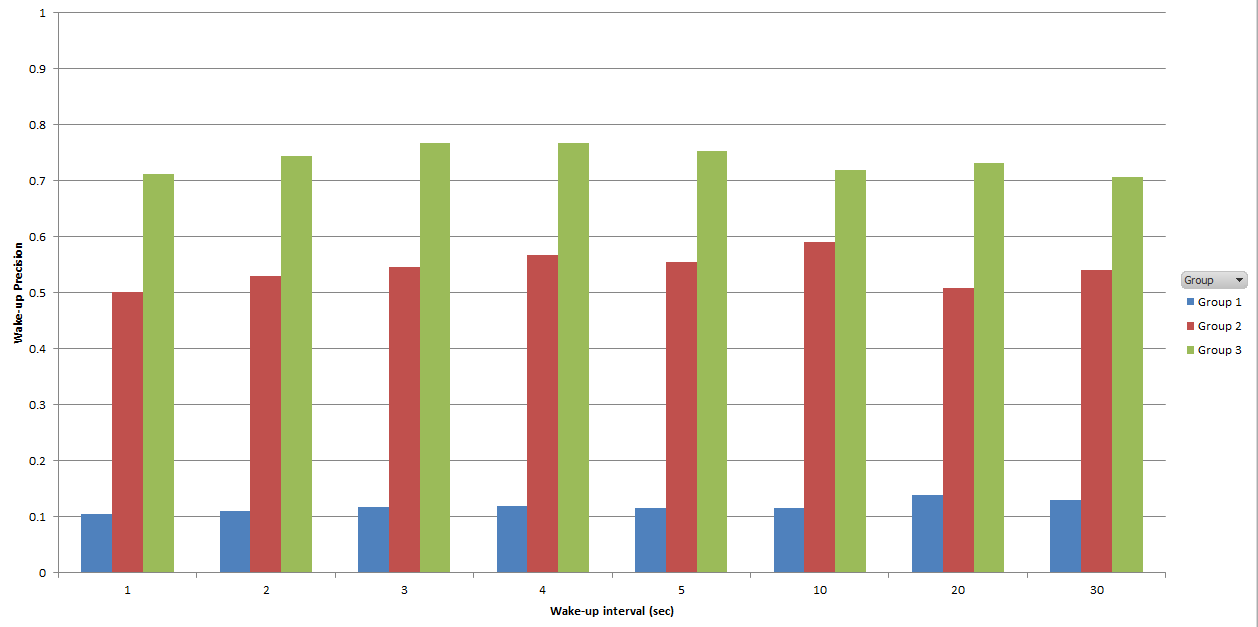
\includegraphics[width=9cm]{dc_wakeup_precision_by_interval.png}
	\caption{Duty Cycling: Wake-up Precision by Wake-up Interval}
    	\label{fig:dcWakeUpPrecisionByInterval}
\end{figure}


\begin{figure}[p]
	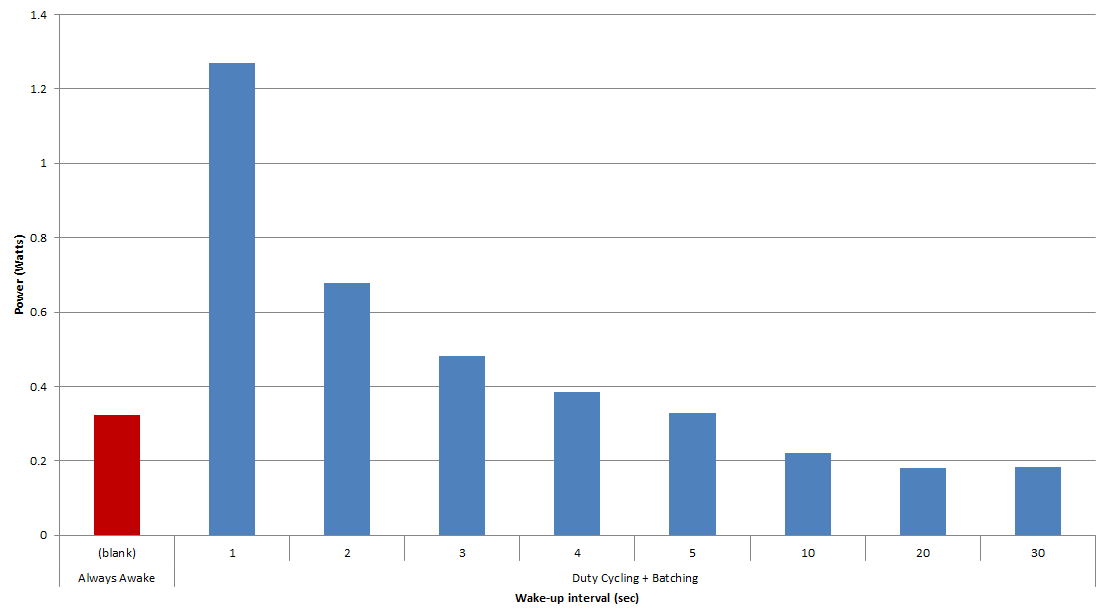
\includegraphics[width=9cm]{batching_power_by_interval.png}
	\caption{Batching and Duty Cycling: Power by Wake-up Interval}
    	\label{fig:batchingPowerByInterval}
\end{figure}


\begin{figure}[p]
	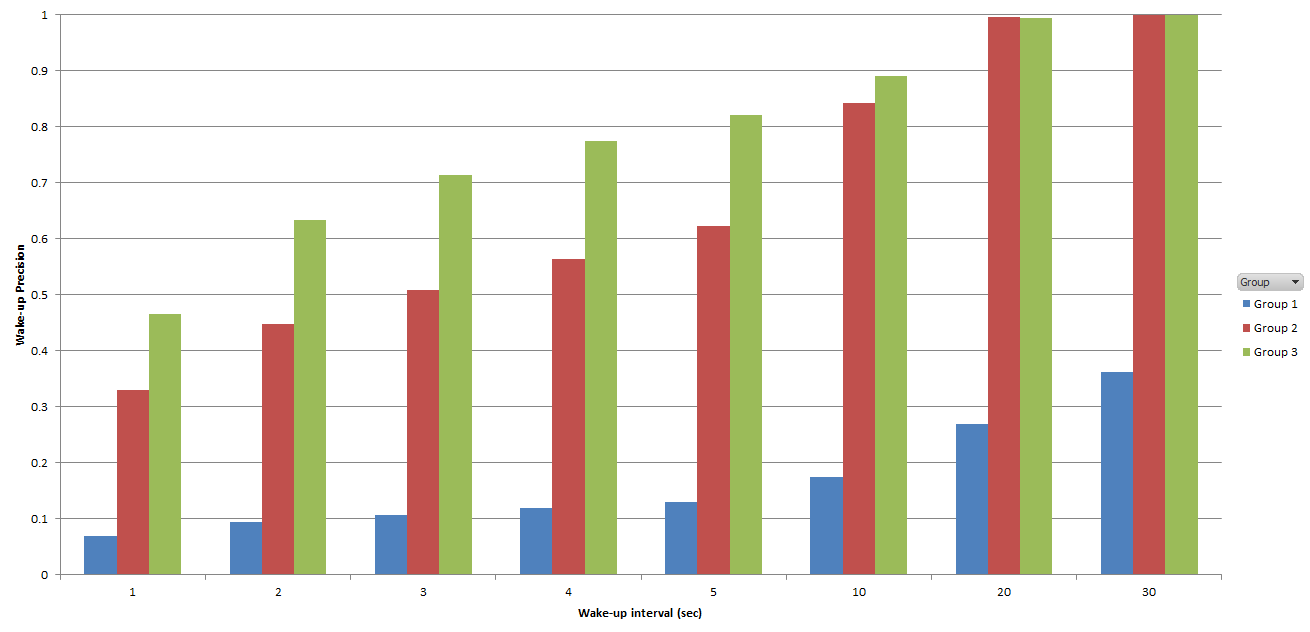
\includegraphics[width=9cm]{batching_wakeup_precision_by_interval.png}
	\caption{Batching and Duty Cycling: Wake-up Precision by Wake-up Interval}
    	\label{fig:batchingWakeUpPrevisionByInterval}
\end{figure}


\begin{figure}[p]
	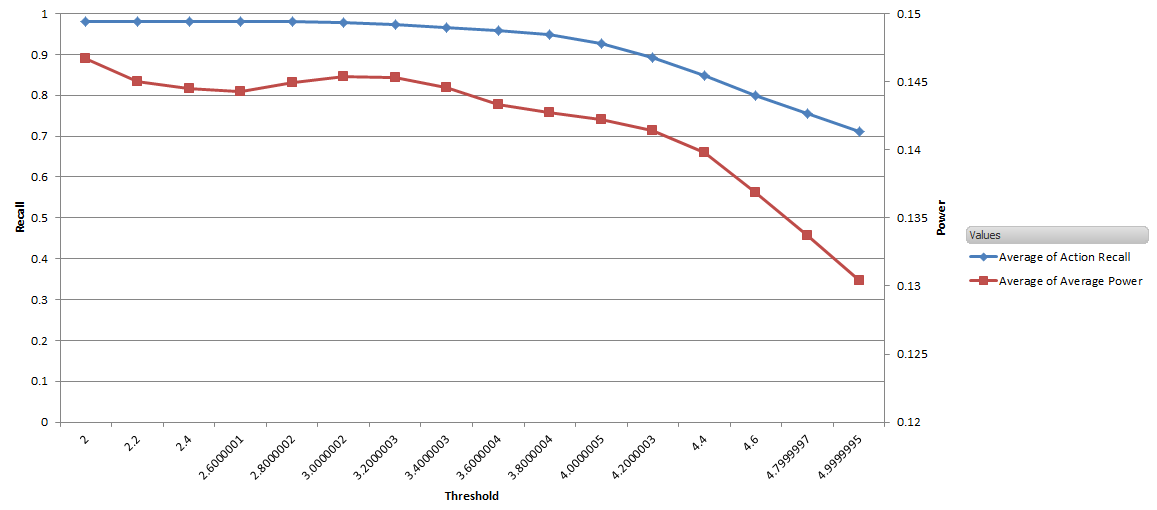
\includegraphics[width=9cm]{wuc_step_th.png}
	\caption{Recall and Power for Wake-up Conditions - Steps - Thresholding}
    	\label{fig:wucStepTh}
\end{figure}


\begin{figure}[p]
	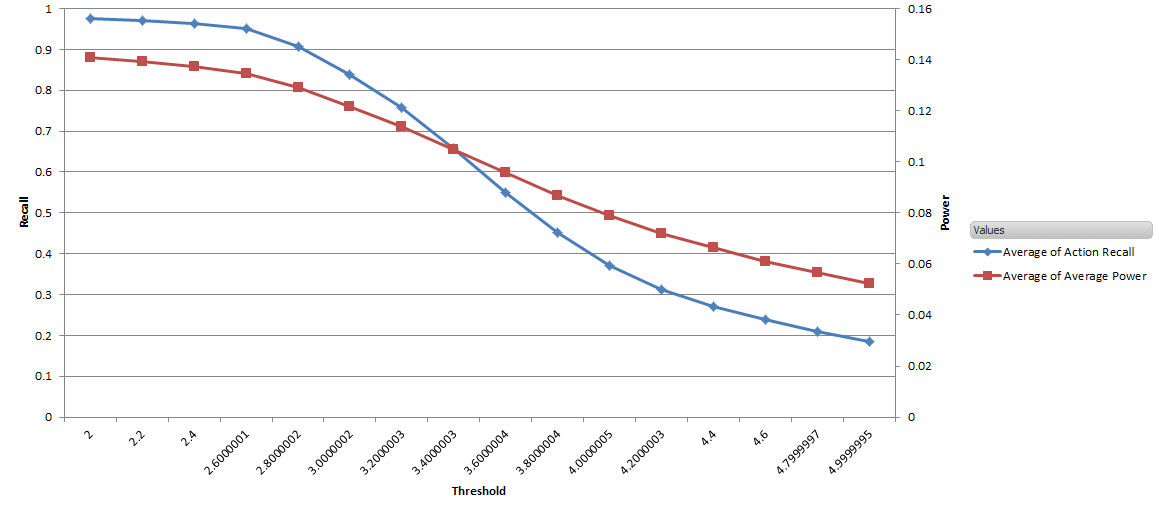
\includegraphics[width=9cm]{wuc_step_ema_th.png}
	\caption{Recall and Power for Wake-up Conditions - Steps - EMA LPF - Threshold}
    	\label{fig:wucStepEmaTh}
\end{figure}


\begin{figure}[p]
	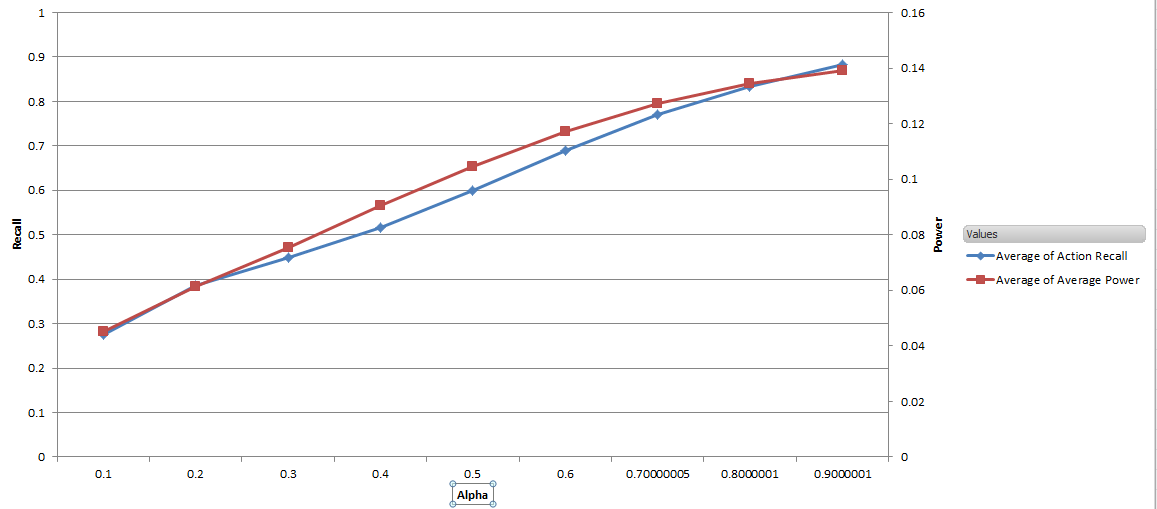
\includegraphics[width=9cm]{wuc_step_ema_alpha.png}
	\caption{Recall and Power for Wake-up Conditions - Steps - EMA LPF - Alpha}
    	\label{fig:wucStepEmaAlpha}
\end{figure}


\begin{figure}[p]
	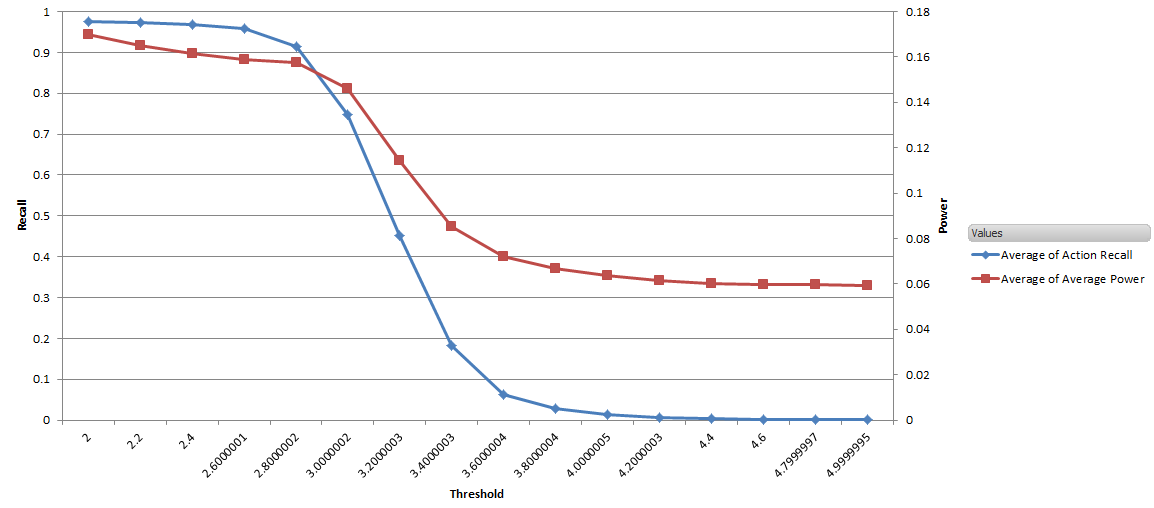
\includegraphics[width=9cm]{wuc_step_fft_th.png}
	\caption{Recall and Power for Wake-up Conditions - Steps - FFT LPF - Threshold}
    	\label{fig:wucStepFftTh}
\end{figure}


\begin{figure}[p]
	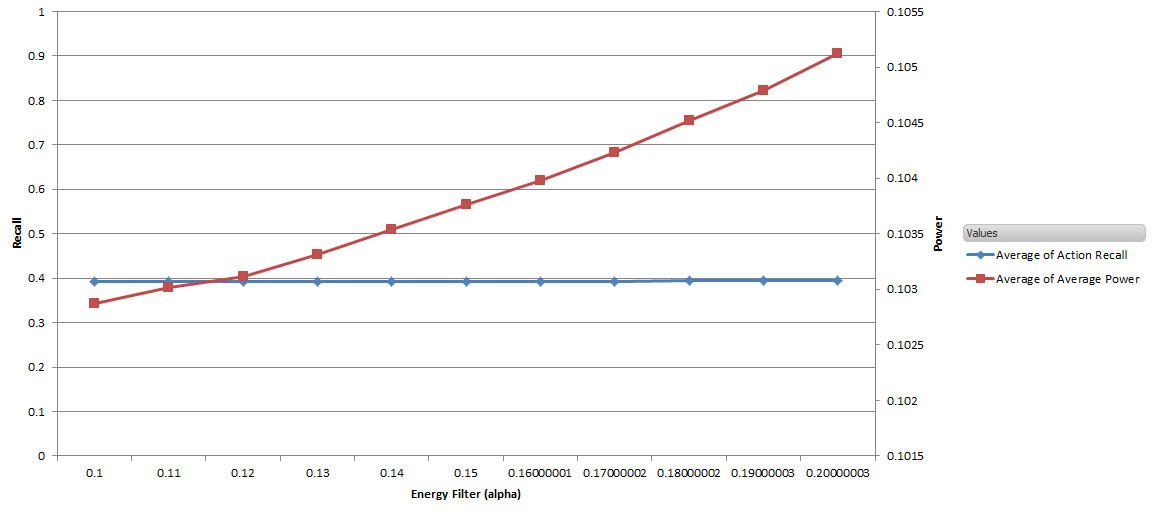
\includegraphics[width=9cm]{wuc_step_fft_alpha.png}
	\caption{Recall and Power for Wake-up Conditions - Steps - FFT LPF - Alpha}
    	\label{fig:wucStepFftAlpha}
\end{figure}


\begin{figure}[p]
	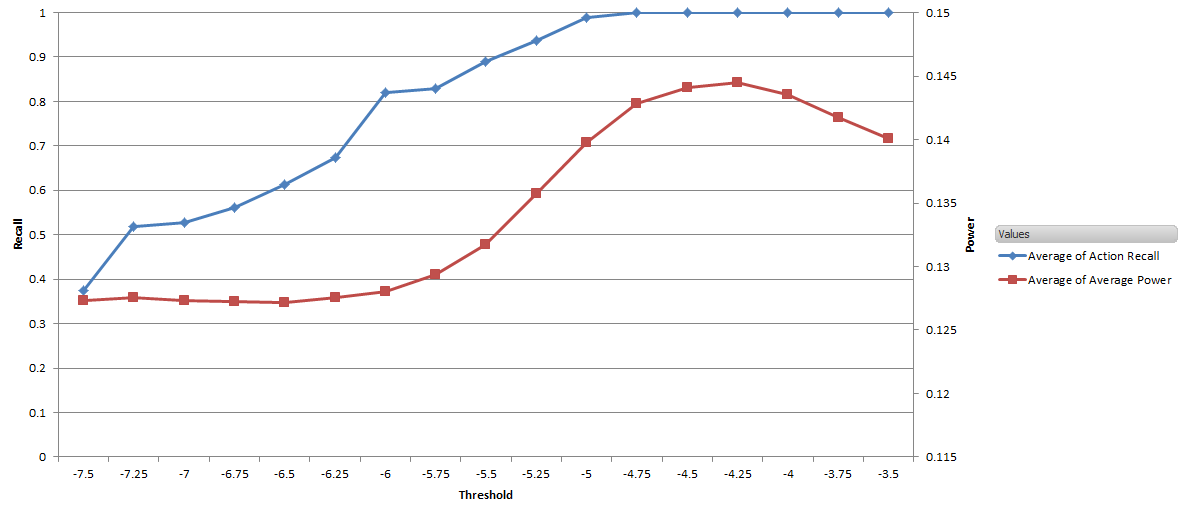
\includegraphics[width=9cm]{wuc_hb_th.png}
	\caption{Recall and Power for Wake-up Conditions - Headbutts - Thresholding}
    	\label{fig:wucHbTh}
\end{figure}


\begin{figure}[p]
	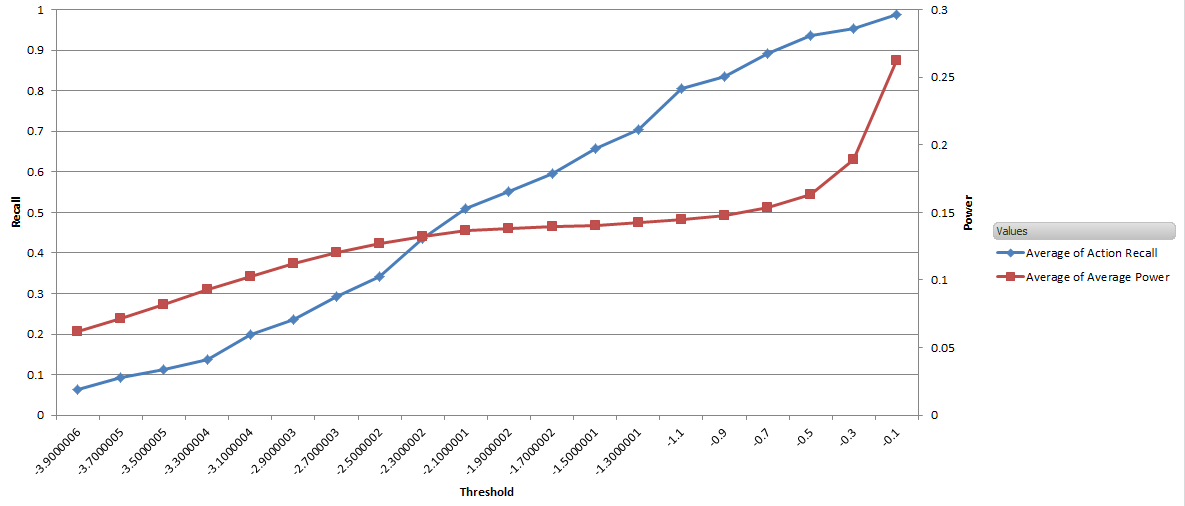
\includegraphics[width=9cm]{wuc_hb_ema_th.png}
	\caption{Recall and Power for Wake-up Conditions - Headbutts - EMA LPF - Threshold}
    	\label{fig:wucHbEmaTh}
\end{figure}


\begin{figure}[p]
	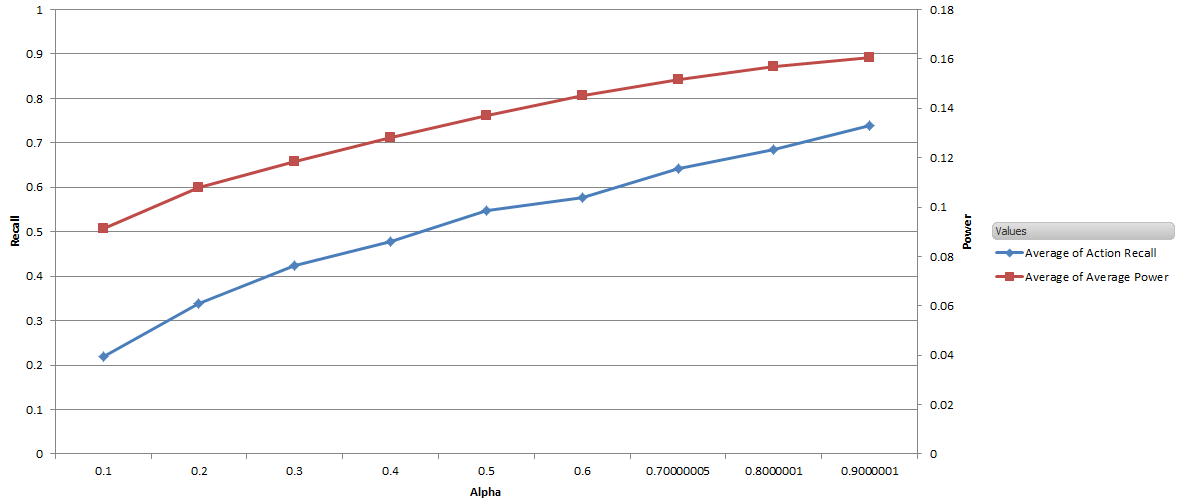
\includegraphics[width=9cm]{wuc_hb_ema_alpha.png}
	\caption{Recall and Power for Wake-up Conditions - Headbutts - EMA LPF - Alpha}
    	\label{fig:wucHbEmaAlpha}
\end{figure}


\begin{figure}[p]
	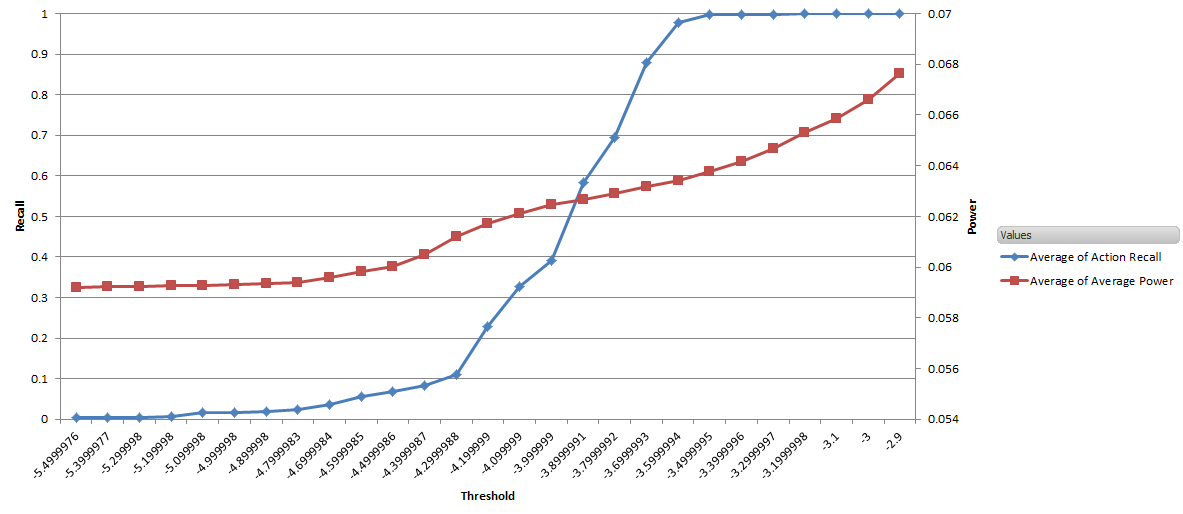
\includegraphics[width=9cm]{wuc_hb_fft_th.png}
	\caption{Recall and Power for Wake-up Conditions - Headbutts - FFT LPF - Threshold}
    	\label{fig:wucHbFftTh}
\end{figure}


\begin{figure}[p]
	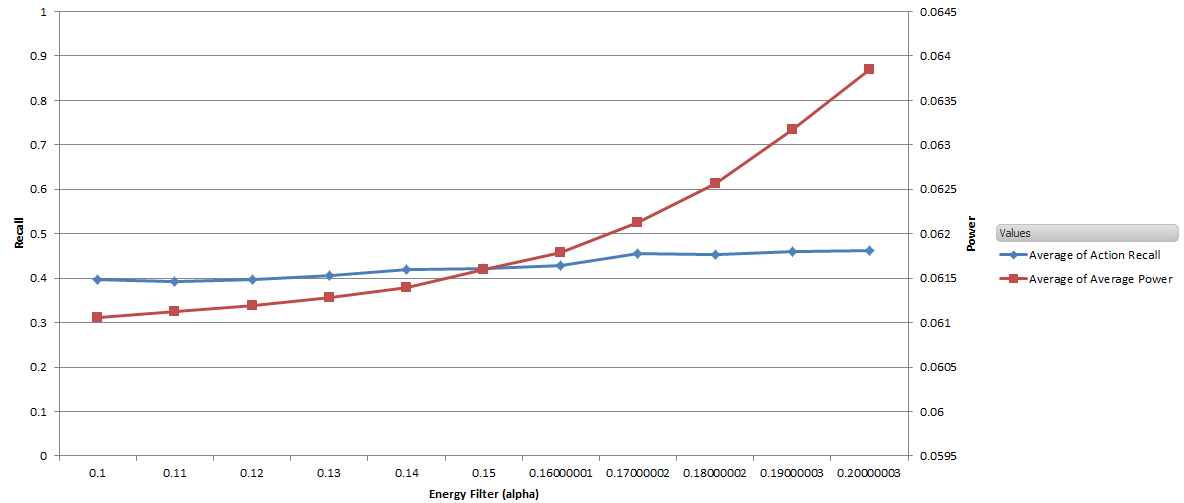
\includegraphics[width=9cm]{wuc_hb_fft_alpha.png}
	\caption{Recall and Power for Wake-up Conditions - Headbutts - FFT LPF - Alpha}
    	\label{fig:wucHbFftAlpha}
\end{figure}

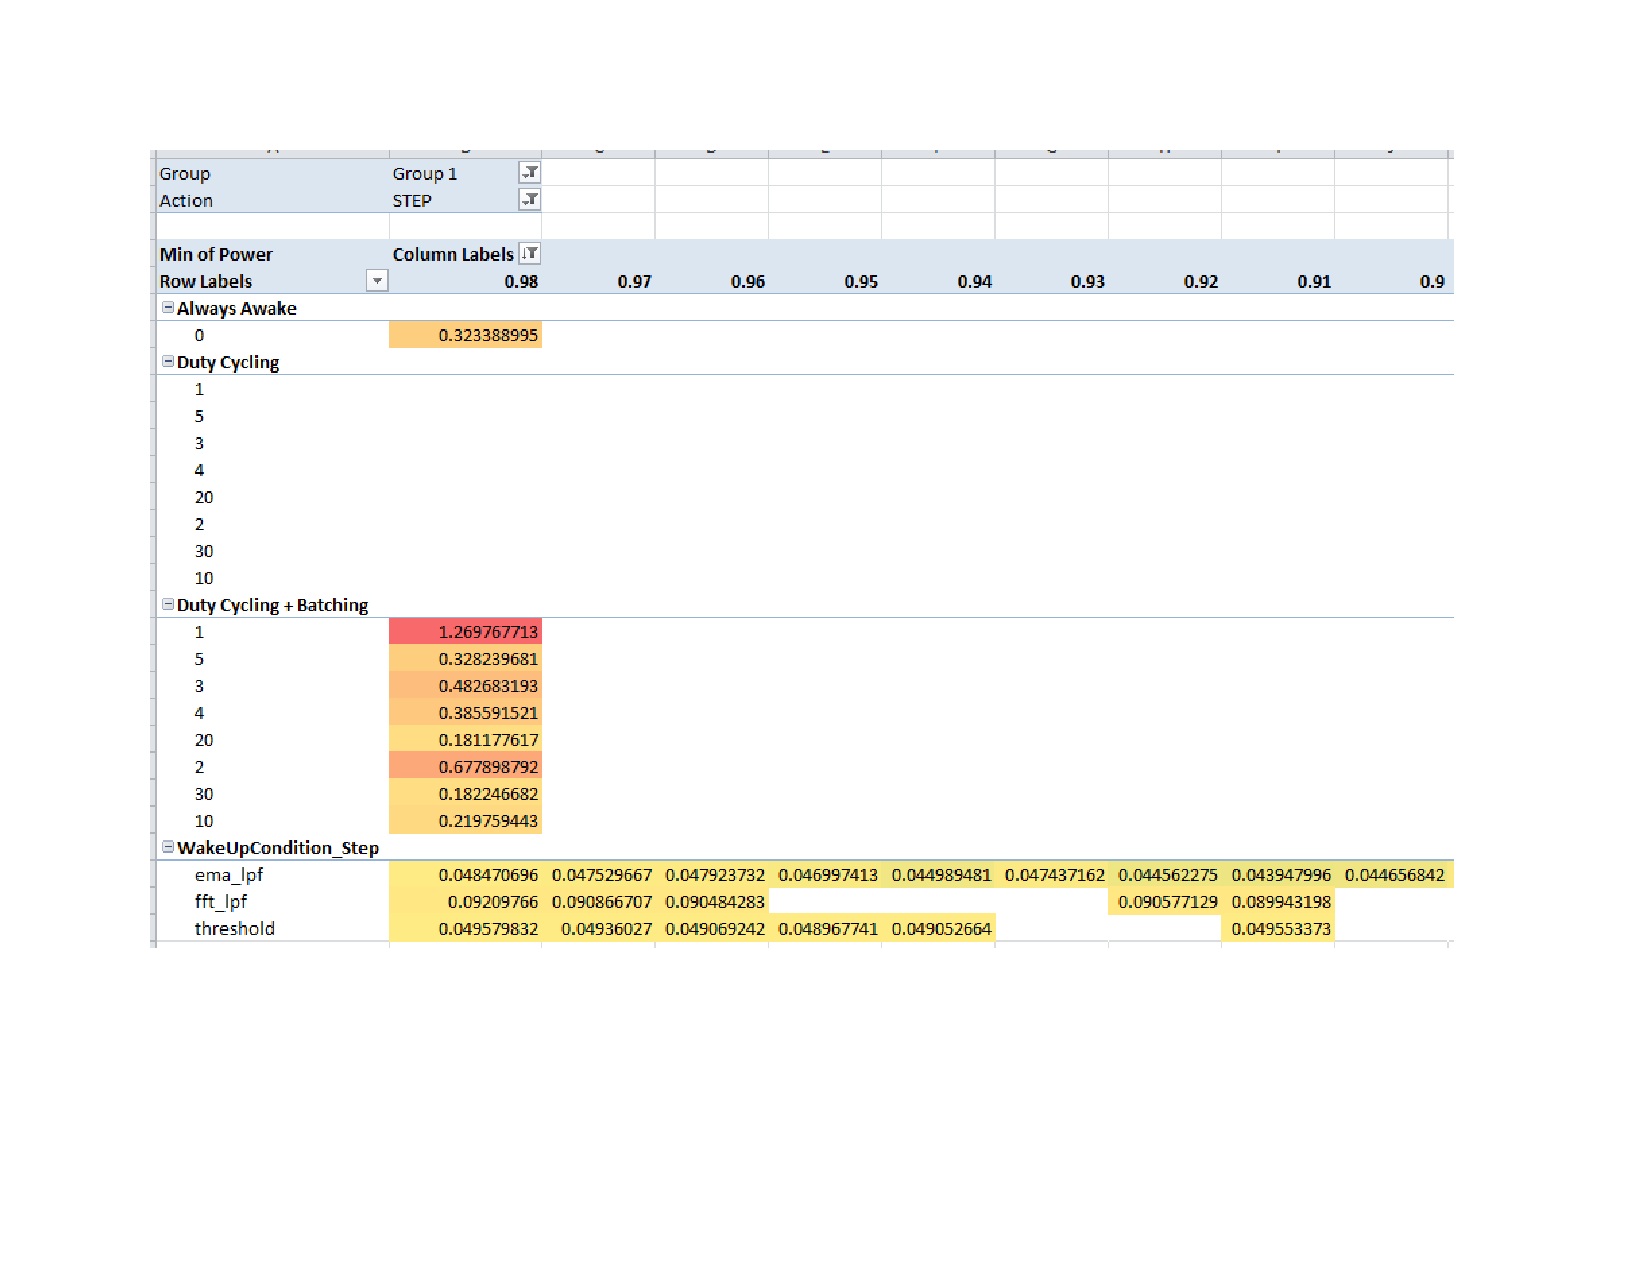
\includepdf[pages={-}]{summaries.pdf}